\chapter{Descripción del Problema}
\label{ch:descprob}
Dada la importancia que tiene la educación en Chile, debido a su magnitud ya que es un tema que aborda a toda la sociedad, y a las constantes entradas y salidas de este sistema, se hace necesario conocer más a fondo los factores que influyen en la deserción escolar, saber cómo se relacionan entre ellos para que así las autoridades correspondientes sepan cómo enfrentarse a este problema.

Para comenzar, es necesario hacer una distinción entre dos conceptos que aparentan ser similares pero que para efectos de este documento no lo son. Estos son deserción y abandono. La deserción escolar se entiende como el retiro temporal o definitivo de un estudiante del sistema educativo. Por otro lado, abandono escolar considera a los estudiantes que se retiran del sistema escolar durante un año académico específico sin evaluar si el retiro es temporal o si el estudiante se reincorpora al siguiente periodo. La deserción escolar considera la salida del sistema escolar como una situación que presenta cierta permanencia en el tiempo\cite{mineduc}.

Antes de comenzar a profundizar el problema que se abarcará y cómo se abarcará, es necesario entender la situación actual de la educación en Chile mediante datos duros.

\newpage

\section{Medición de la Deserción en Chile}

El Ministerio de Educación de Chile, mediante su Centro de Estudios, ha creado un documento llamado Serie Evidencias, que constituye un nuevo aporte a la generación de espacios de discusión y reflexión en base a evidencia científica. En estos documentos se abordan tópicos relevantes para el área de la educación.

En Marzo de 2013 se presentó una \textit{Medición de la deserción escolar en Chile}. Para esto se presentan dos tasas de mediciones de deserción escolar\cite{serieevidencias}:

\begin{description}
  \item[Tasa de Incidencia] \hfill \\
  Mide la deserción escolar evaluando la transición de un año a otro, por lo que se considera desertor al alumno que no retorna al sistema escolar luego de hacer estado matriculado en el periodo académico anterior, sin que durante este periodo se haya graduado del sistema escolar. 
  La importancia de este indicador radica en la rapidez con que es posible determinar a los desertores del sistema, lo que permite aplicar políticas focalizadas a este grupo de alumnos.\\
  Matemáticamente, en Chile esta tasa se define de la siguiente manera:\\
  
  \begin{center}
$TDI_t^j = \frac{Des_{t}^{j}}{Des_{t}^{j} + M_{t}^{j}}$
    \end{center}
Donde:
\begin{itemize}[label=]
    \item $TDI_t^j$: tasa de deserción medida como incidencia en el grado $j$ y periodo $t$.
    \item $Des_{t}^{j}$: corresponde al número de personas que desertaron del sistema escolar en el grado $j$ y periodo $t$
    \item $M_{t}^{j}$: corresponde a la matrícula efectiva en abril del periodo $t$ y grado $j$.
\end{itemize}

\newpage

    Además, el número de personas que desertaron del sistema escolar en un grado y año dado, se define como continúa.

  \begin{center}
  $Des_{t}^{j} = Ap_{t-1}^{j-1} + Rep_{t-1}^{j} + Ret_{t-1}^{j}$\\
    \end{center}
Donde:
\begin{itemize}[label=]
    \item $Des_{t}^{j}$: corresponde al número de personas que desertaron del sistema escolar en el grado $j$ y periodo $t$.
    \item $Ap_{t-1}^{j-1}$: corresponde a quienes, habiendo aprobado el grado $j-1$ en el periodo $t-1$, no presentan matrícula en el periodo $t$, sin que durante este periodo hayan finalizado la educación escolar.
    \item $Rep_{t-1}^{j}$: corresponde a quienes habiendo reprobado el grado $j$ en el periodo $t-1$, no presentan matrícula en el periodo $t$.
    \item $Ret_{t-1}^{j}$: corresponde a quienes se retiraron durante el periodo $t-1$, en el grado $j$, y no presentan matrícula en el periodo $t$.
\end{itemize}


\item[Tasa de Prevalencia] \hfill \\
  Evalúa la deserción escolar desde una perspectiva estática ya que considera el estado presente de la persona analizada, y no la trayectoria educacional que ésta ha tenido. Permite conocer la proporción de jóvenes que no terminaron la educación escolar y que tampoco se encuentran matriculados en ningún establecimiento educacional en el periodo analizado.
  La ventaja de la utilización de esta medida es que posibilita la comparación con oros sistemas educativos, y al mismo tiempo entrega una visión del fenómeno en un rango temporal más amplio, lo que permite un monitoreo a largo plazo.
  Matemáticamente, en Chile esta tasa se define de la siguiente forma:\\
   
   \begin{center}
$TDP_t^j = \frac{P_{t}^{j} - M_{t}^{j} - G_{t}^{j} - NA_{t}^{j}}{P_{t}^{j} - NA_{t}^{j}}$
    \end{center}
Donde:
\begin{itemize}[label=]
    \item $TDP_t^j$: corresponde a la tasa de deserción, medida
como prevalencia, en el periodo $t$ para el rango de edad $j$.
    \item $P_{t}^{j}$:  corresponde a la población total del rango de edad $j$, en el periodo $t$.
    \item $M_{t}^{j}$: corresponde a la población en el rango de edad $j$ que no ha concluido sus estudios escolares, pero asiste a un establecimiento educacional.
    \item $G_{t}^{j}$: corresponde a la población en el periodo $t$, en el rango de edad $j$, que concluyó sus estudios escolares.
    \item $NA_{t}^{j}$: población que, en el periodo de tiempo $t$ y rango de edad $j$, nunca ha asistido a la educación escolar.
\end{itemize}
\end{description}

Luego de estas definiciones, se procederá a evidenciar la situación del abandono escolar en Chile según los datos de la encuesta CASEN\footnote{Encuesta de Caracterización Socioeconómica Nacional, es una encuesta a nivel nacional, regional y comunal, que realiza el gobierno de Chile desde el año 1985. Esta encuesta es mandatada por el Ministerio de Planificación y Cooperación (MIDEPLAN) y se caracteriza por medir las condiciones socio-económicas de los hogares del país, en términos de acceso a la salud, la educación, el trabajo y a las condiciones de la vivienda.}

Un detalle importante, antes de entrar a las cifras de deserción, es hacer una diferenciación entre tasas globales y tasas del sistema regular. Esta última considera que el universo utilizado está compuesto sólo por educación básica y educación media, a diferencia de las tasas globales, que además de estos dos niveles considera un tercero que es la educación de adultos, a la que pertenecen quienes no terminaron la educación básica o media y pretender terminarla con 18 años o más. 

Entonces, para efectos de este proyecto, el foco será la tasa de deserción del sistema regular. 

Procediendo a los resultados que presenta el Centro de Estudios del MINEDUC, la tasa de deserción del sistema regular para el periodo 2011 es de 3\%, lo que equivale a 91.968 personas que presentaban matrícula el año 2011 y no se gradúan ni se encuentran matriculados en el sistema regular de educación de niños y jóvenes el año 2012. A continuación se muestra la tasa de deserción por grado en el año 2011. 

\begin{figure}[H]
  \centering
    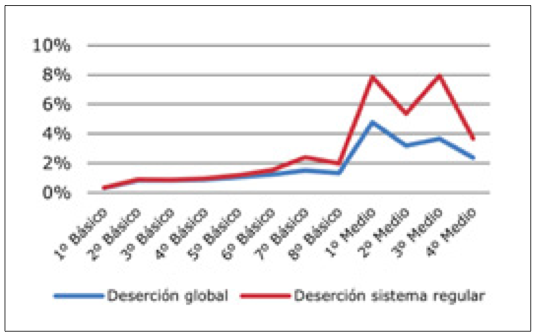
\includegraphics[width=0.7\textwidth]{Figuras/desercioncurso}
      \caption{Tasa de Incidencia de la deserción por Curso, 2011. Fuente: MINEDUC}
    \label{fig:curso}
\end{figure}

En base a la Figura~\ref{fig:curso}, es posible notar que las tasas son mayores en la educación media, generándose un quiebre en el paso de educación básica a la media. Un punto importante a considerar para este quiebre es que un número importante de establecimientos educacionales sólo imparten enseñanza básica, lo que obliga a los estudiantes a buscar otro establecimiento, y esto aumenta la probabilidad de deserción escolar. 

También se genera una diferencia por género, donde los hombres presentan una tasa de deserción del sistema regular del 3,3\%, sin embargo para las mujeres se obtiene un 2,7\%.

Otro punto importante que se presenta es la existencia de mayores tasas en establecimientos municipales, cuya tasa de deserción del sistema regular es del 3,8\%. Para el caso de los particulares pagados, se observan las menores tasas de deserción del sistema regular, con un 0,3\%. En la Figura~\ref{fig:admin} se muestran estas tasas con mayor detalle.

\begin{figure}[H]
  \centering
    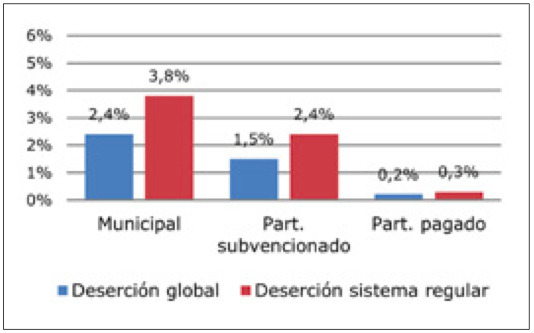
\includegraphics[width=0.7\textwidth]{Figuras/desercionadmin}
      \caption{Tasa de Incidencia de la deserción escolar según dependencia administrativa, año 2011. Fuente: MINEDUC}
    \label{fig:admin}
\end{figure}

\section{Conclusiones}

Debido a que el foco del presente trabajo es la deserción escolar, lo que se propone es la creación de un sistema de alerta temprana de la deserción escolar para el sistema público, específicamente en la Región Metropolitana. 
El fin de este sistema de alerta temprana no es en ningún caso reemplazar la toma de decisiones, sino que apoyar este proceso. Estas decisiones son aquellas relacionadas con la creación de políticas públicas referentes al área de educación en Chile, pero específicamente las decisiones que afectan directamente al área de la educación pública. 

La creación de un Sistema de Alerta Temprana se refiere a un instrumento de predicción basado en procedimientos estandarizados de obtención, análisis y procesamiento de datos relativos a la educación pública, destinado a alertar a los centros de decisión política para la adopción de medidas que eviten o atenúen el problema a tiempo. 

Dentro de los procedimientos a considerar para la creación de este Sistema de Alerta Temprana se requiere comenzar por conocer el contexto de la educación pública actual en Chile, para luego seleccionar las fuentes de información con que se trabajará e identificar, mediantes diferentes análisis, cuáles son los factores que desencadenan la deserción escolar. Con esto ya se puede dar el siguiente paso, que es generar procedimientos estandarizados mediante Minería de Datos que permitan visualizar los focos de deserción.